\documentclass[twoside]{report}

\usepackage{project}

\begin{document}

\begin{titlepage}
  %\vspace{12cm}
	\raggedright
  {\Large{\colorbox{front}{\color{white} \textbf{NORRSKEN}\kern 1pc}}\\\vspace{0.3cm}}
  {\texttt{Project Plan}\\}
  \vfill
	{\large \today\par}
  {\small\color{gray} ID: Marc Coquand, Linus Lagerhjelm, Mattias Cederberg and Simon
  Asp\\}
  {\small\color{gray} OT: Catarina Berglund, Sofie Abrahamsson\\}
  {\small\color{gray} Supervised by Stig Byström}\\
  {\small\color{gray} Umeå University, done in collaboration with Umeå
  Municipality. Contact: Carina Aschan, carina.aschan@umu.se\\}

	%\vfill

\end{titlepage}

\newpage
\pagecolor{front}\afterpage{\nopagecolor}\thispagestyle{empty}

\marginpar{\textcolor{white}{\small{\texttt{Project
Management}}\vspace{11cm}\\\large\textbf{Summary}\\ {\small 
Walking home late at night can be a daunting experience. The newspapers write
about assaults and harassment, the northern winter climate contribute with
shorter days and darker nights. Existing street lights helps with the problem
but the feeling of uncertainty and fear persist. Norrsken will investigate
how a technical solution could be applied to create an increased sense of
safety. The project is carried out in collaboration with the municipality of
Umeå and Umeå University as part of the courses Interactivity in Smart
Environments and Project Management.
}}} 
 \newpage

\tableofcontents
\thispagestyle{empty}
\newpage


\section{Introduction}
\subsection{Purpose}
Design a proposal for a safe smart city environment where individuals’ personal
preferences and needs are met, build a demonstrator and, maybe, translate the
solutions to rural areas.
\subsection{Background}

Walking home late at night can be a daunting experience. The newspapers write
about assaults and harassment, the northern winter climate contribute with
shorter days and darker nights. Existing street lights helps with the problem
but the feeling of uncertainty and fear persist. This project will investigate
how a technical solution could be applied to increase safety. It is carried out
in collaboration with the municipality of Umeå and Umeå University as part of
the courses Interactivity in Smart Environments and Project Management.

Smart environments’ purpose is to either improve abilities, control something
or reduce/minimise unwanted events. It can therefore be interesting to see if
the technology can be applied to the problem of security in urban environments. 

In particular smart city technology, wearable computing or sensor networks can
perhaps be used to solve the problem of security. 

\subsection{Goals} The goal is to, before December 15th, produce a concept as
well as a model of a knowledge domain for a smart environment that, by being
proactive and by considering the user's personal preferences, makes the user’s
stay at the campus area safer.
\newpage

\section{SWOT Analysis}

%\begin{figure}[H]
  %\caption{The SWOT analysis}
\marginpar{
  \captionof{figure}{SWOT analysis}
  \begin{tabular}{|p{9cm}|}
    \hline
    Strengths\\  
    \begin{itemize}
      \item  Extensive technical knowledge
      \item  `Fresh eyes' on the problem
      \item  2 Occupational therapist project members
      \item  USP: Increasing safety by creating a more interesting city
    \end{itemize}\\\hline
    Weaknesses\\
    \begin{itemize}
      \item No budget
      \item Insufficient time
      \item Low amount of experience in the specific area
    \end{itemize}\\\hline
    Opportunities 
    \begin{itemize}
      \item Use of equipment in designated project room
      \item Course supervisors and mentors
      \item An increasing trend of technological infrastructure
    \end{itemize}\\\hline
    Threats
    \begin{itemize}
      \item Group member peripheral projects
    \item Required technical equipment might not be available in time
    \end{itemize}\\\hline
  \end{tabular}
}
\begin{leftsiderules}
The SWOT analysis enlightens certain pressure points and gaps for the
project. The group members’ technical knowledge strength can be matched with
the technical equipment opportunity. The limited experience in the area can be
assisted by the course mentors which should provide a greater chance of success.
The lack of budget could be problematic, but for this project all the required
material should be provided, however there is a waiting time for materials that
need ordering. The fact that the project aims to increase safety by making the
city more interesting should be received positively by users and stakeholders in
comparison of a surveillance-centered solution.
\end{leftsiderules}

\subsection{Limitations} The main limitation in the project is that it will
only model a concept for a system. No actual system will be concretised beyond
the model described in the goals-section. Furthermore, the solution proposal
will only take the campus and surrounding areas with the the current residents
into consideration.

\subsection{Delimitations}
Our focus is only on the university area of Umeå. We will also limit us to only making a proof of concept.

\subsection{Aim and Research Questions}

How can these smart environments (stretching over Ålidhem), and these
individuals’ activities be enriched with interactive, intelligent technology
for increasing safety? 

Some interesting questions to solve also as part of this
problem is: How can we increase safety? How can we prototype a smart
environment? What possibilities are there to make the campus and surrounding
environment smart? 

\subsubsection{Anticipated Design Solution that will be Demonstrated January 10-11}

The demonstration will consist of a prototype and a proof of concept. It will then be presented with a live performance.  

\marginfig{graphics/intressent-analys.pdf}{The stakeholder analysis}
\section{Stakeholder Analysis \& Organisational Structure}
\begin{rightsiderules}
As shown in the image, our core stakeholders is the supply
group. They are the ones that has the main interest in completing the project
and also has the most influence over the project. Our primary stakeholders is
the same as the projects clients, i.e. the municipality of Umeå.
Lastly, the secondary stakeholders. Those who will be affected by the project
somehow but will not take part in any decision making within the project.
\end{rightsiderules}

\begin{rightsiderules}
The figure clarifies how the communication should flow through the project. The
project group make sure that they know everything they need to know from he
project owner (Helena at the Interaction in Smart Environments course). They
will also, together with the occupational students, communicate with the
stakeholders at the municipality. In the project group, it is the project leader
that makes sure that all the project members do what they are suppose to. Also
the project group will talk to the OT-students to clear up uncertainties.
\end{rightsiderules}
\captionof{figure}{Organisational structure}
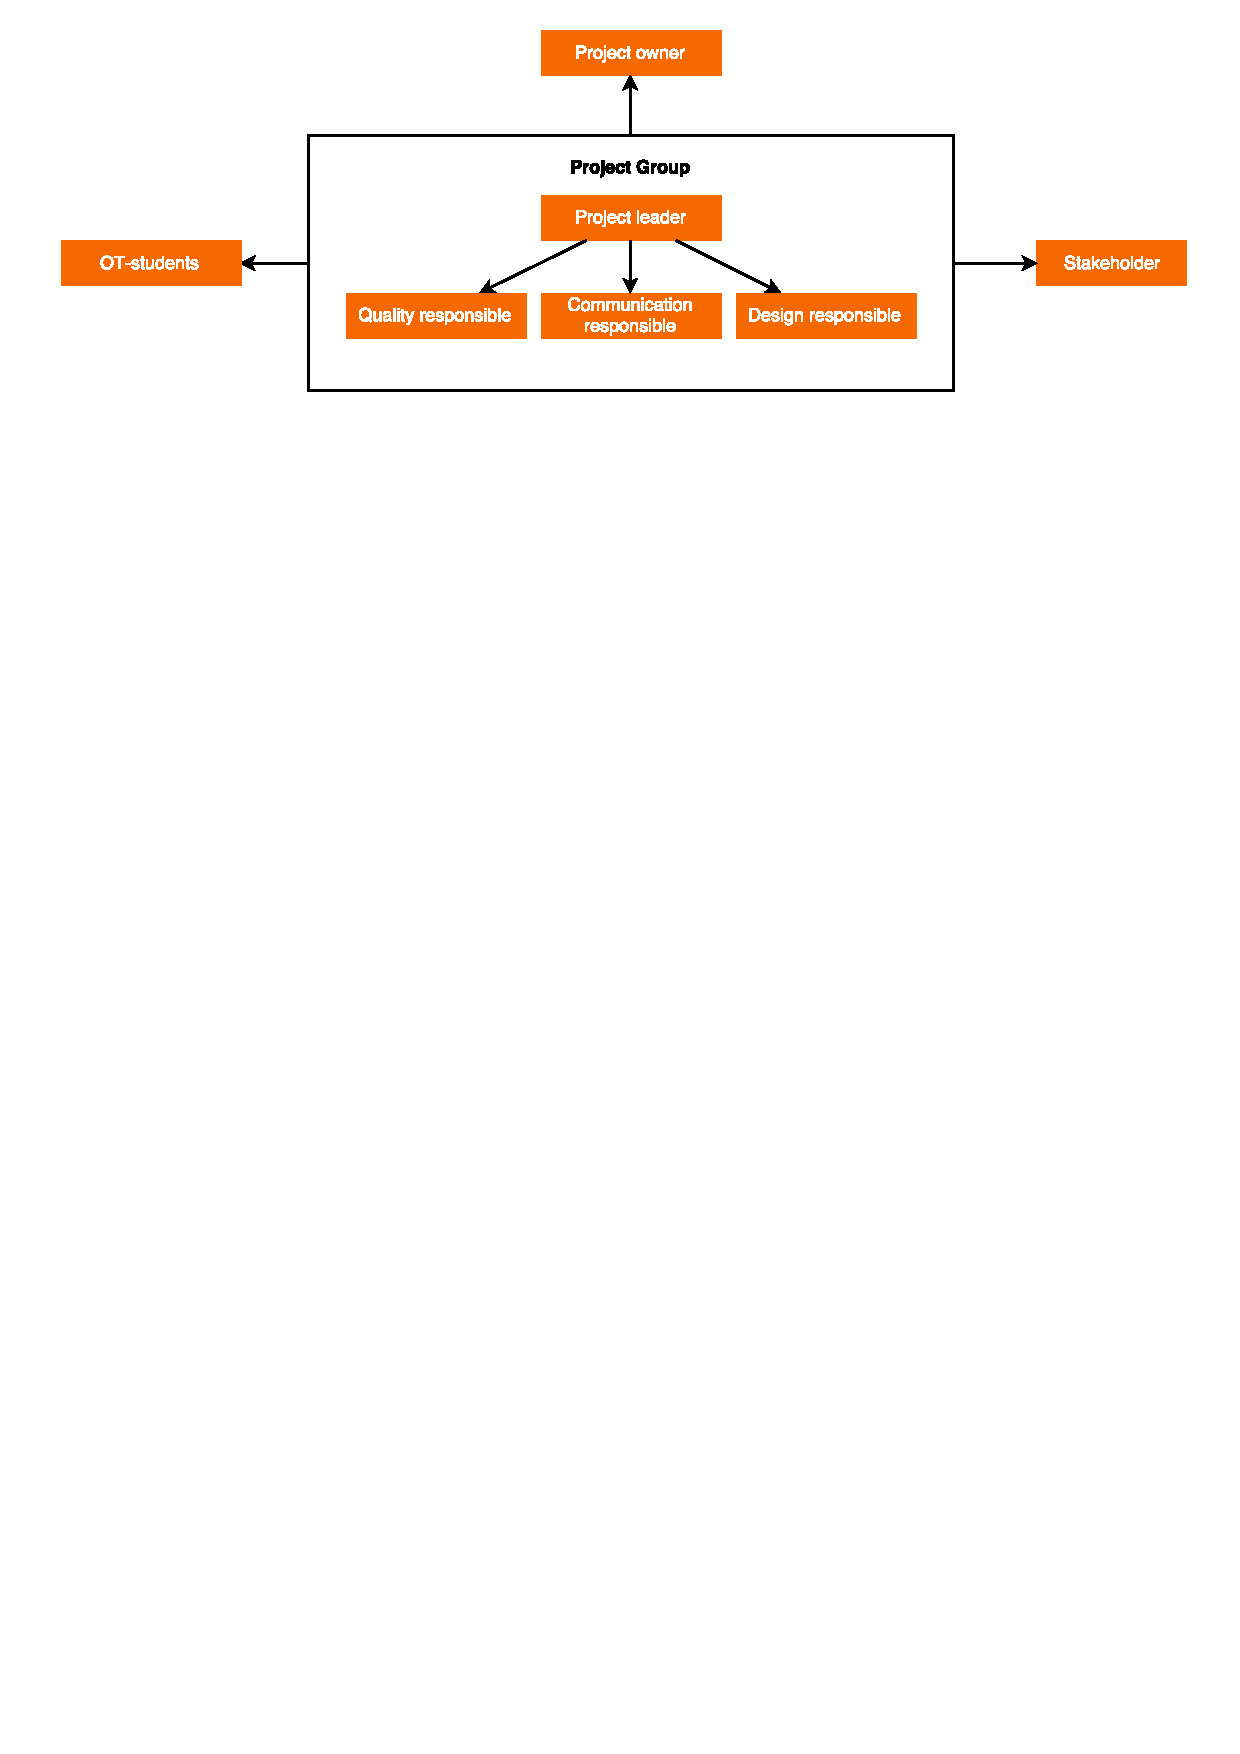
\includegraphics[width=\linewidth]{graphics/Organizationaldiagram.pdf} 



\newpage
%\end{figure}

\section{Work Breakdown Structure (WBS)}
\marginpar{The Work Breakdown Structure shows the breakdown of the work that has
to done. It shows all the essential steps that have to be performed to complete
the task.}
\begin{figure}[H]
  \makebox[\linewidth]{
  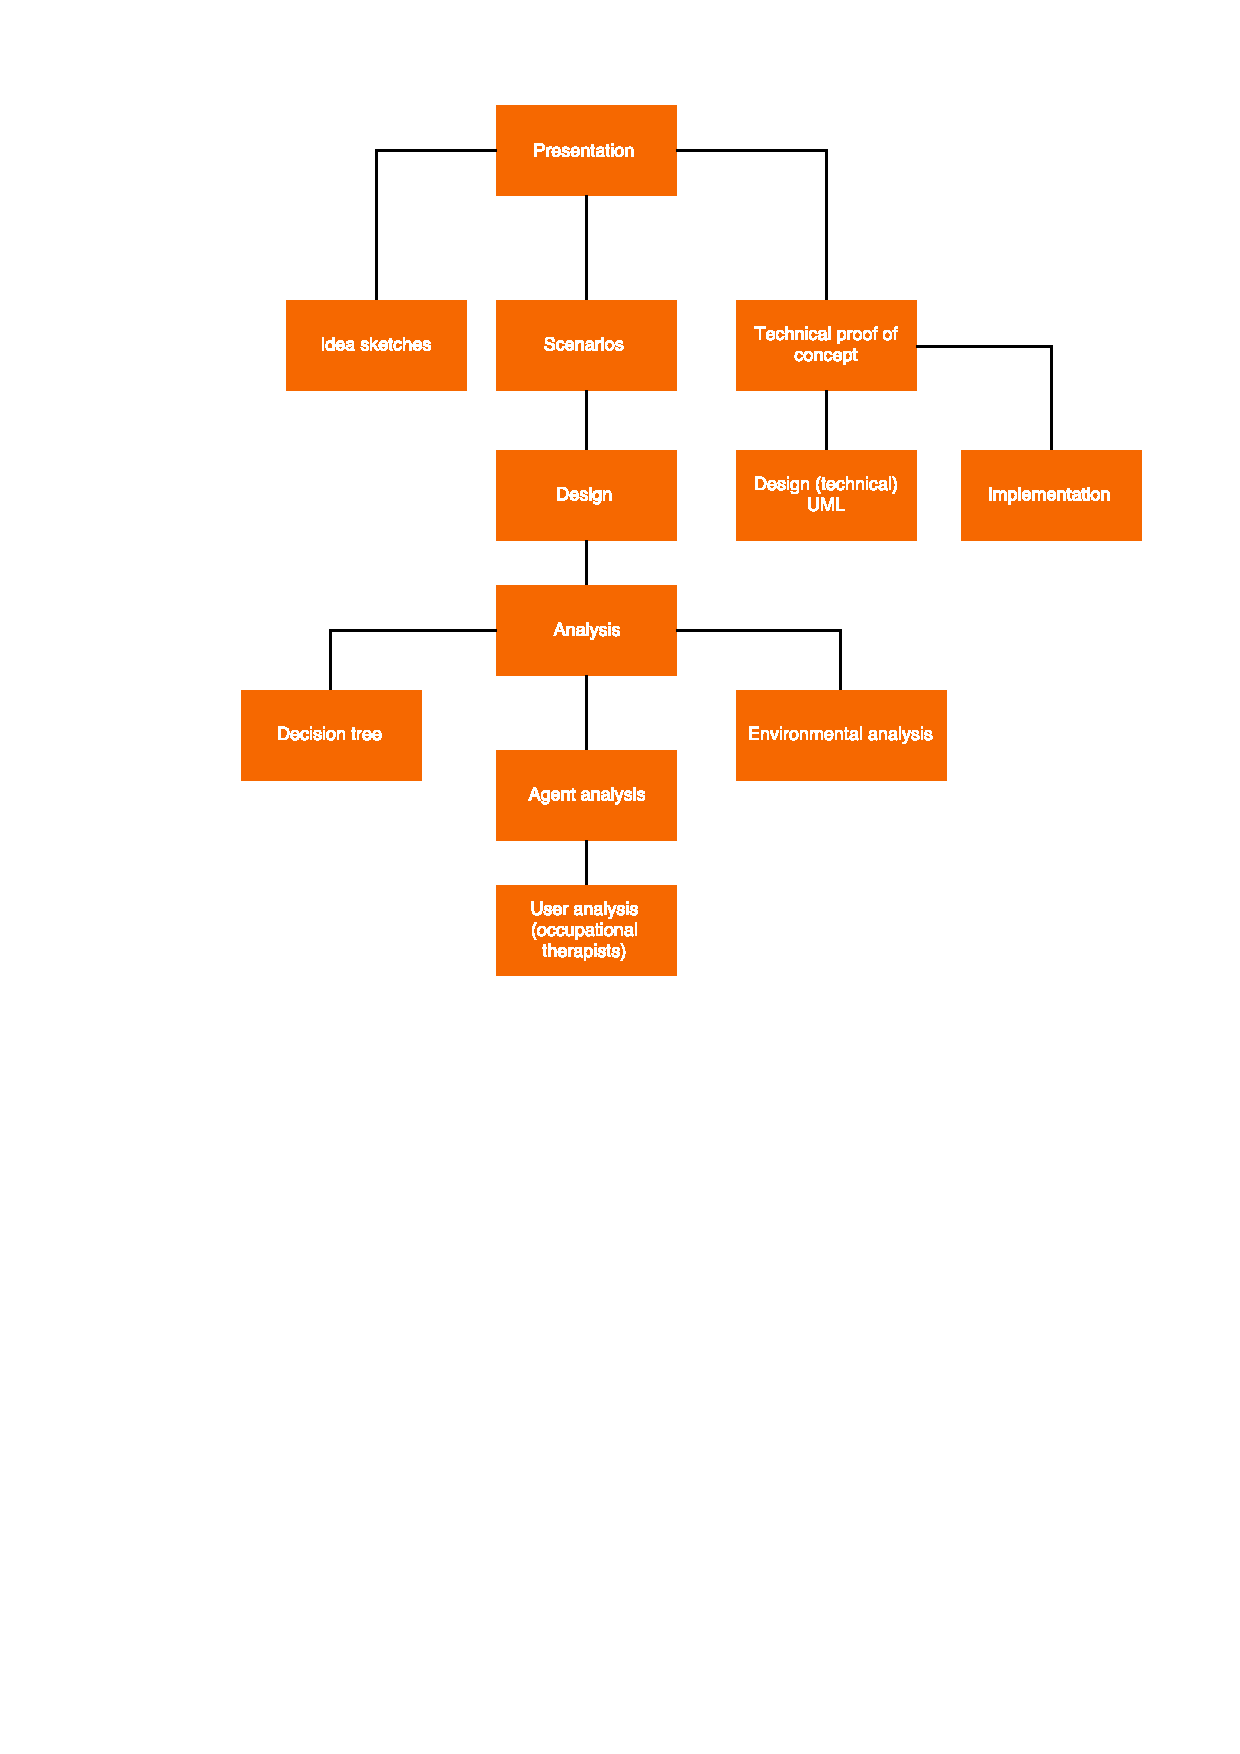
\includegraphics[width=\linewidth]{graphics/wbs.pdf} 
  }
  \caption*{}
\end{figure}

\section{Communication Plan \& Document Plan}

\subsection{Communication Plan}

\captionof{figure}{Communication plan}
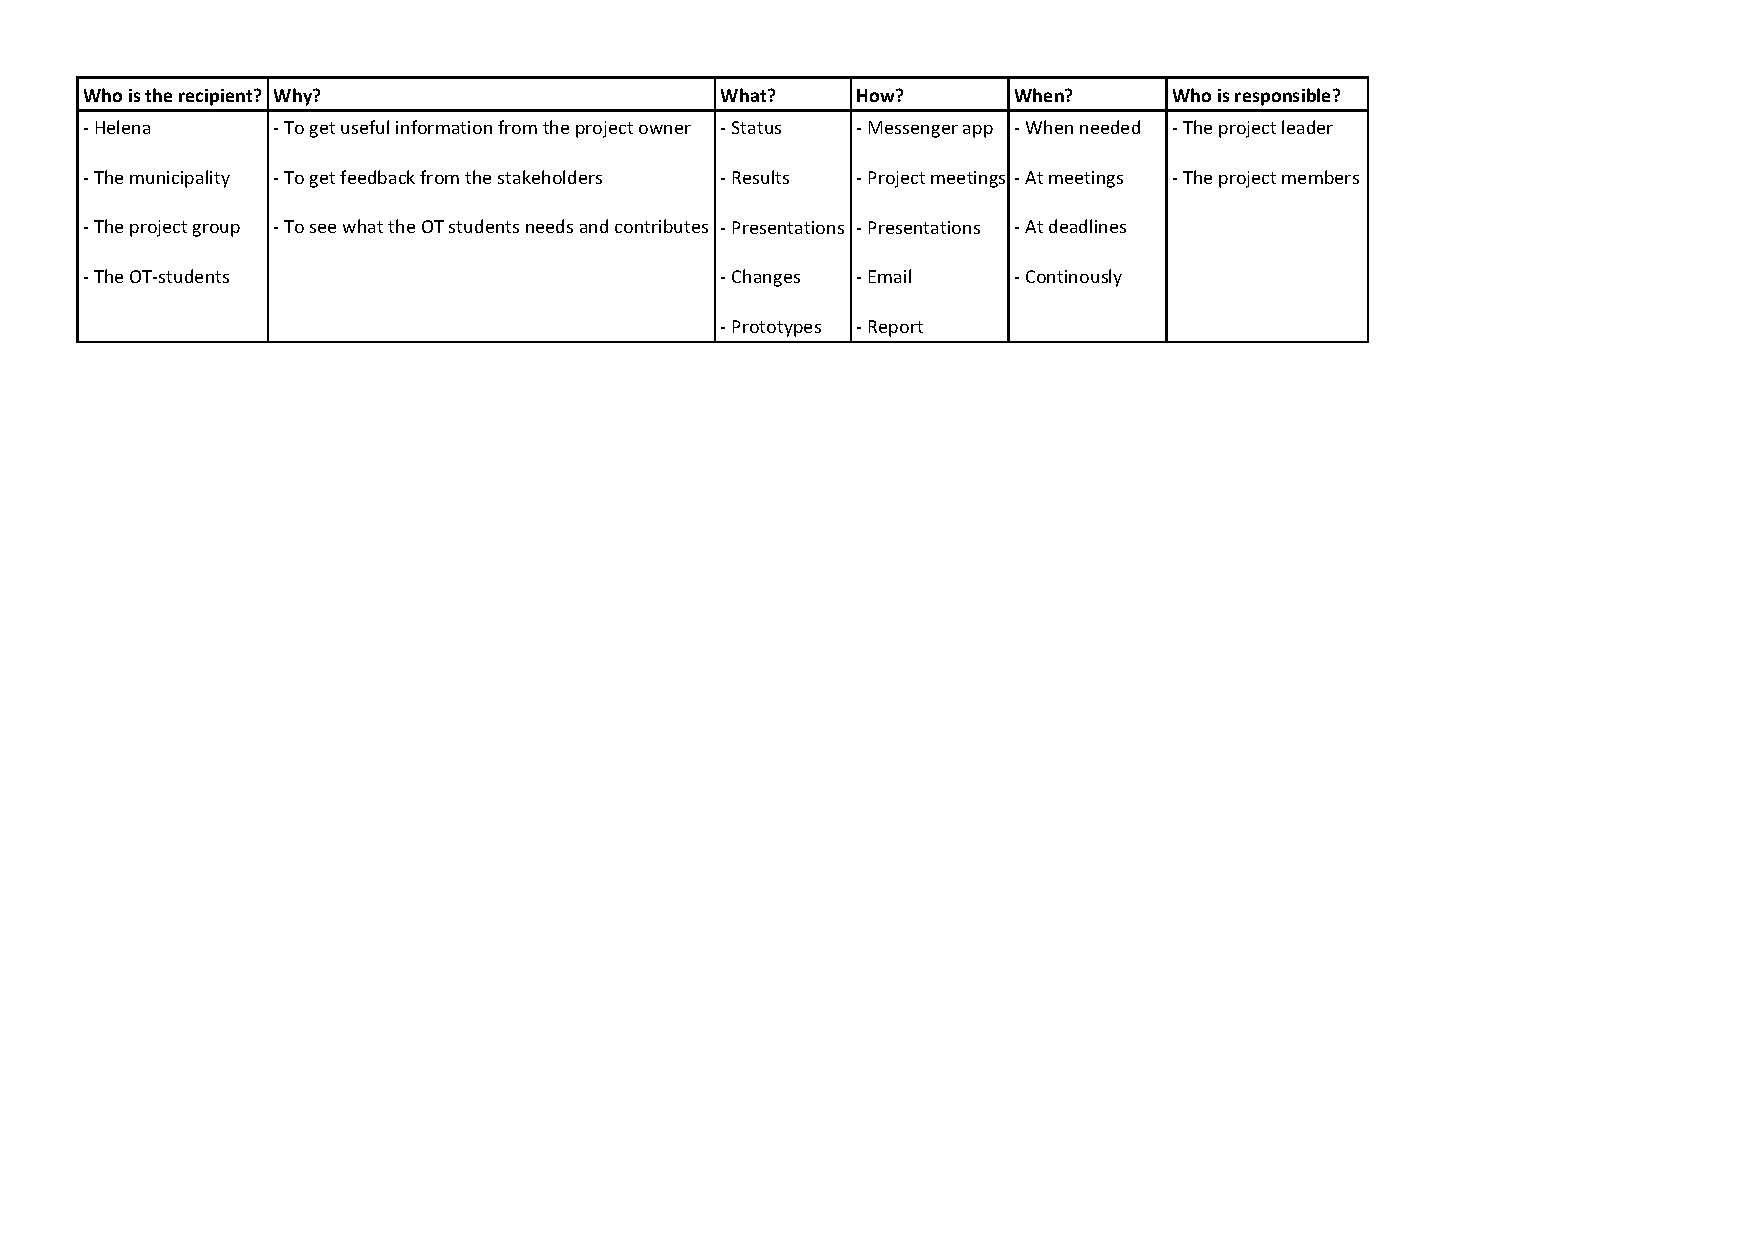
\includegraphics[width=\linewidth]{graphics/communcationplan.pdf} 

\subsection{Document Plan}
All documents are written in English and stored digitally in the Google Drive
shared by all project members. The structure is as such that all pictures that
can be used for the purpose of documentation and articles are stored in their
respective folder in the resource folder. 

All project management content is stored in their respective folder: pilot study
and project plan, presentations, journal and meetings. The agenda for the
meetings and making sure the journal is written is the responsibility of the one
responsible for the documents, I.E. Marc. 

All the documents that are sent to non-group members must follow a fixed latex
template, for the pilot study and project plan it’s Marc’s responsibility to
fix so the document follows the template. 

\newpage
\section{Milestones}

\captionof{figure}{Milestones}
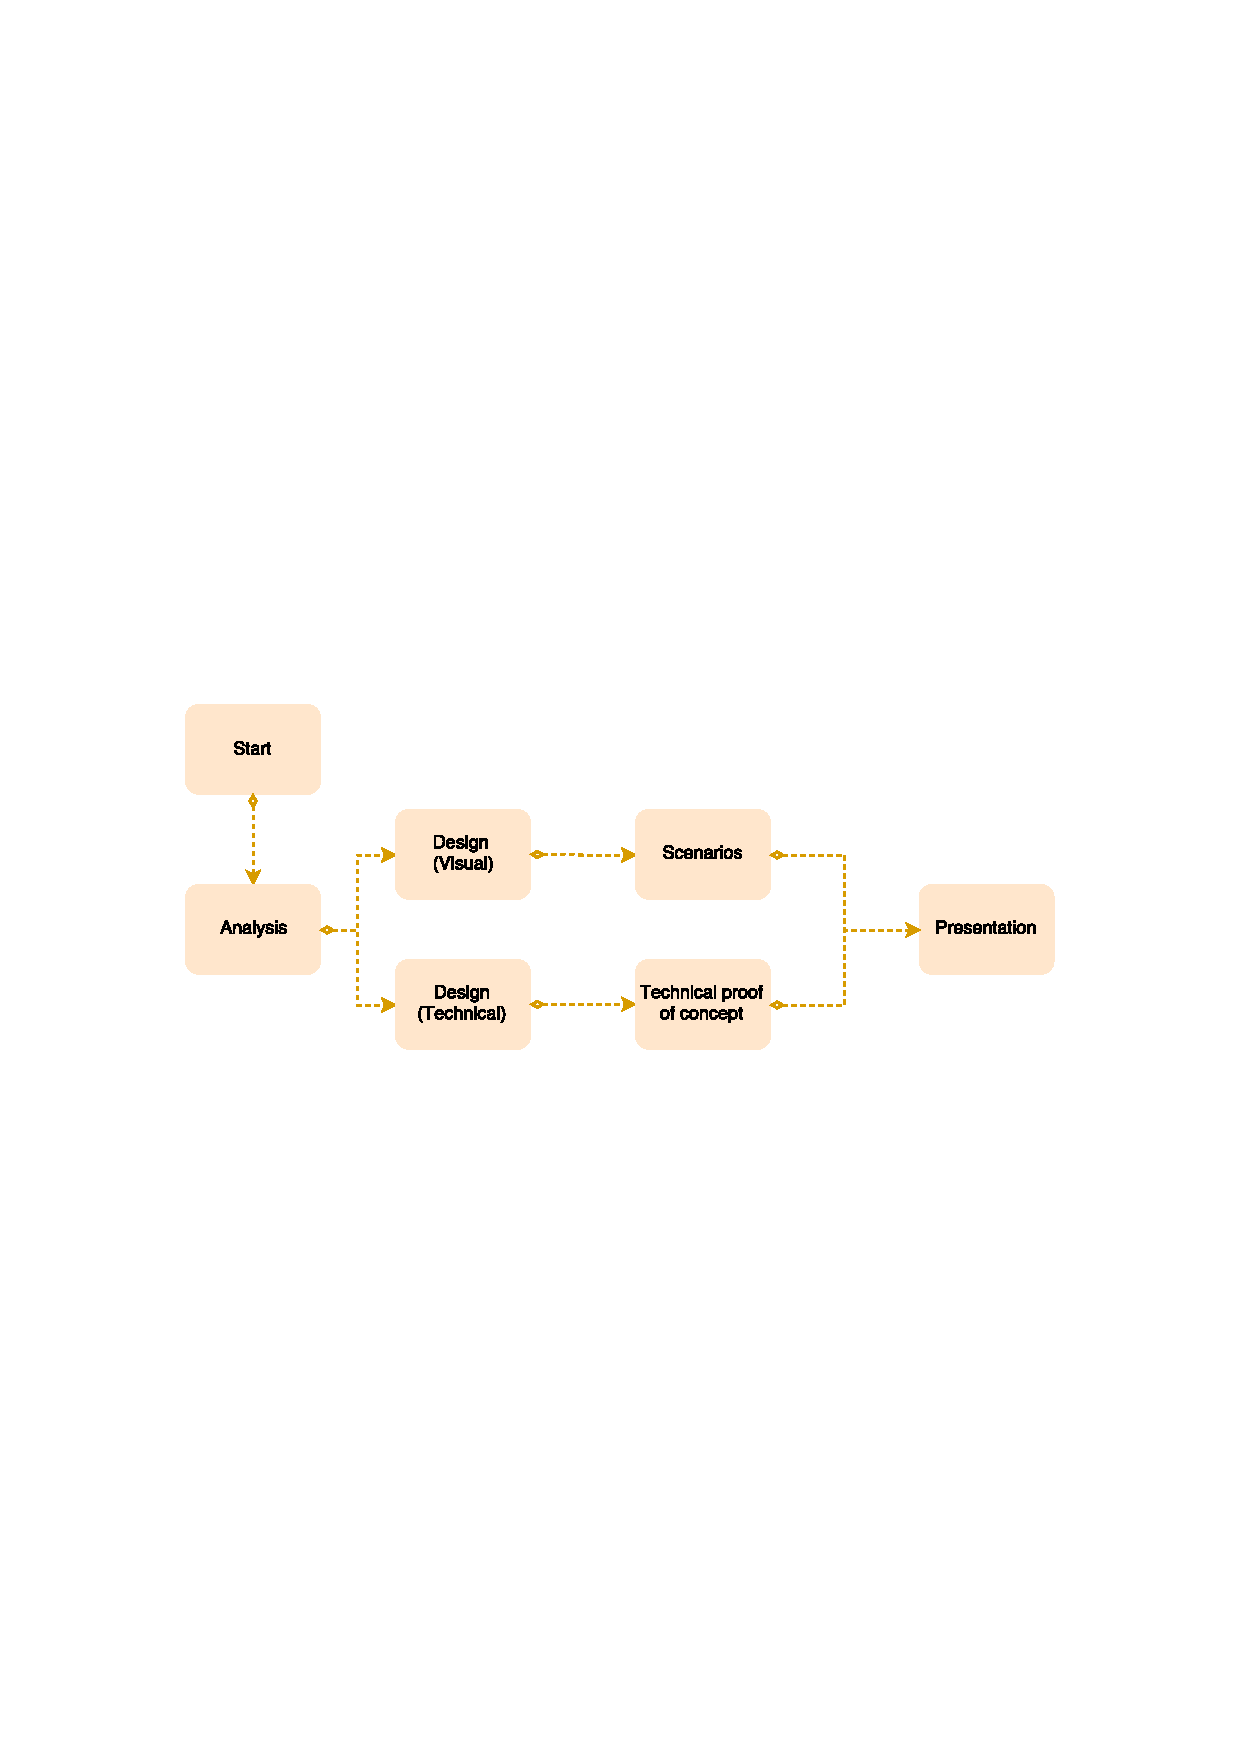
\includegraphics[width=\linewidth]{graphics/Milestones.pdf} 

\section{Time Plan - Gantt}
The time schedule serves the purpose of determining how the project is
progressing time-wise. It consists of four milestones: 

Milestone 1: Analysis of the user, environment and software agent of the system.
Milestone 2: Technical design in the form of a decision tree and a UML class
\marginpar{\textbf{UML} \color{gray}{ (Unified modeling language) is a tool used 
by programmers for modeling the system so that it's easier to implement.}}
diagram. Visual in the form of concept art. Milestone 3: User scenarios and a
technical proof of concept. Milestone 4: Presentation and technical report.

As the project progresses and a milestone is reached, the previous work is to be
evaluated before the project group can move on to the following work
packages. The first milestone is the analysis phase. The given problem is
evaluated and the project structure is developed. This has to be completed in
order for the next block of work packages can be tackled: the design. 

The design of the solution in terms of functionality and visual features are
developed with regards to the previous analysis work. The behaviour of the
system is structured with a decision tree and a UML class diagram. The visual
aspect of it will be represented with concept art. 

As the design phase is complete, the project group are able to move on to
building the technical proof of concept and creating user scenarios. It is
essential that the design is fully developed before this phase is initiated. For
the proof of concept the technical design is required and for the user scenarios
the interaction aspect of the system needs to be developed. 

When milestone 3 passes evaluation, the final phase can be commenced. It
consists of the project presentation and a technical report describing the
different parts of the project. It is essential that this milestone is completed
before the presentation deadline; 11 of January 2016.
\captionof{figure}{Gantt Chart}
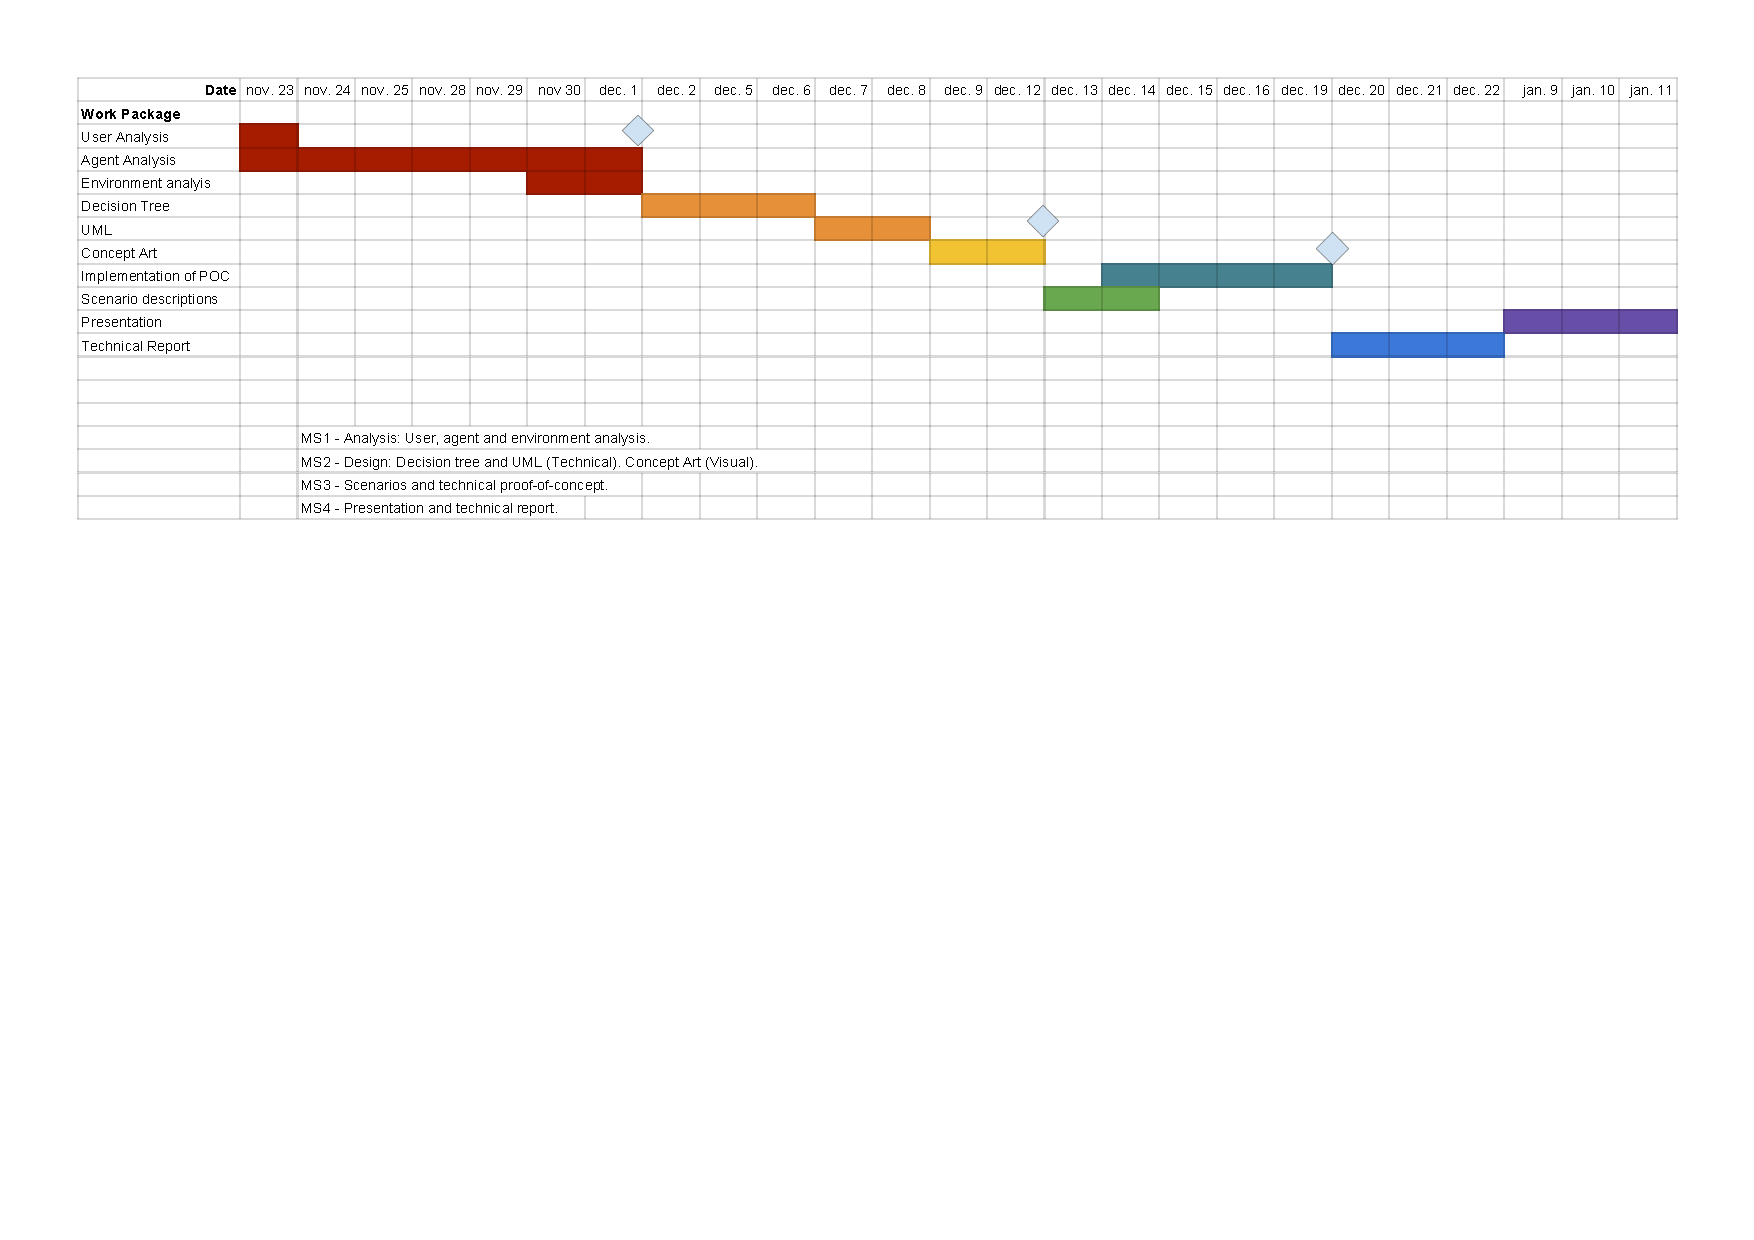
\includegraphics[scale=0.9]{graphics/gantt.pdf} 

\section{Risk analysis}

\subsection{Identification}

The biggest danger to this project is the time constraints. The project has to
be presentable on December the 15 and complete January the 11. The biggest
threat is the lack of clear structure in the specification given by the teacher
as well as limited technical knowledge. Overall anything unclear can make it
difficult to be compliant with the time estimation. It’s also important to
watch out for potential problems with the scenario descriptions and sketches as
they might not fulfill their purpose, I.E. explaining the product. 

\subsection{Evaluation}

The mini-method risk gives us.

\begin{tabular}{|l|l|l|l|}
  \hline
  Scenario & Probability & Consequence & Risk value \\\hline
  Not done in time & 1 & 1 & 1 \\\hline
  Implementation issues & 2 & 2 & 4 \\\hline
  Unclear specification from teacher & 3 & 2 & 6 \\\hline
\end{tabular}

\subsection{Action Plan}

The biggest hurdle to not being done in time is implementation issues and
unclear specification from teachers. The action plan is then to be in constant
contact with the teachers and supervisors, instead of wasting time trying to
comprehend unclear instructions. As far as the projects sketches are concerned
the way to avoid it is to have a strict review procedure with the entire group
as well as evaluating if it’s comprehensible for people who are outside of the
project group. 

\newpage
\section{Activity List}
\captionof{figure}{Activity List. OT - Ocupational Therapists, PG - Project
Group, PL - Project Leader, D - Design Responsible, C - Communication Responsible
, Q - Quality Responsible}
\includegraphics[scale=0.9]{graphics/activity.pdf} 

\section{Resources and Budget}
The project goal is a presentation consisting of concept art describing the
design and interaction of the system and a proof of concept describing some of
its technological features. Due to the nature of the project, material costs
will be able to be kept on a minimum and the vast majority of the outlay will be
in the form of working hours. The ID-students will have the role of developers
during the course of the project. They will have to spend more hours on the
project and will therefore be the largest expense. The OT-students will assist
by sharing their knowledge of their specific area and by contributing with
valuable data by producing surveys. The OT-students part of the project will be
the most intense during the onset of the project. 

As for the specific cost of the different resources the costs are as such:

Lead developer: 740 kr/h a 58h
Developer: 517 kr/h a 174h
Assistant: 240 kr/h a 26h
Material/Sensors: 5000 kr

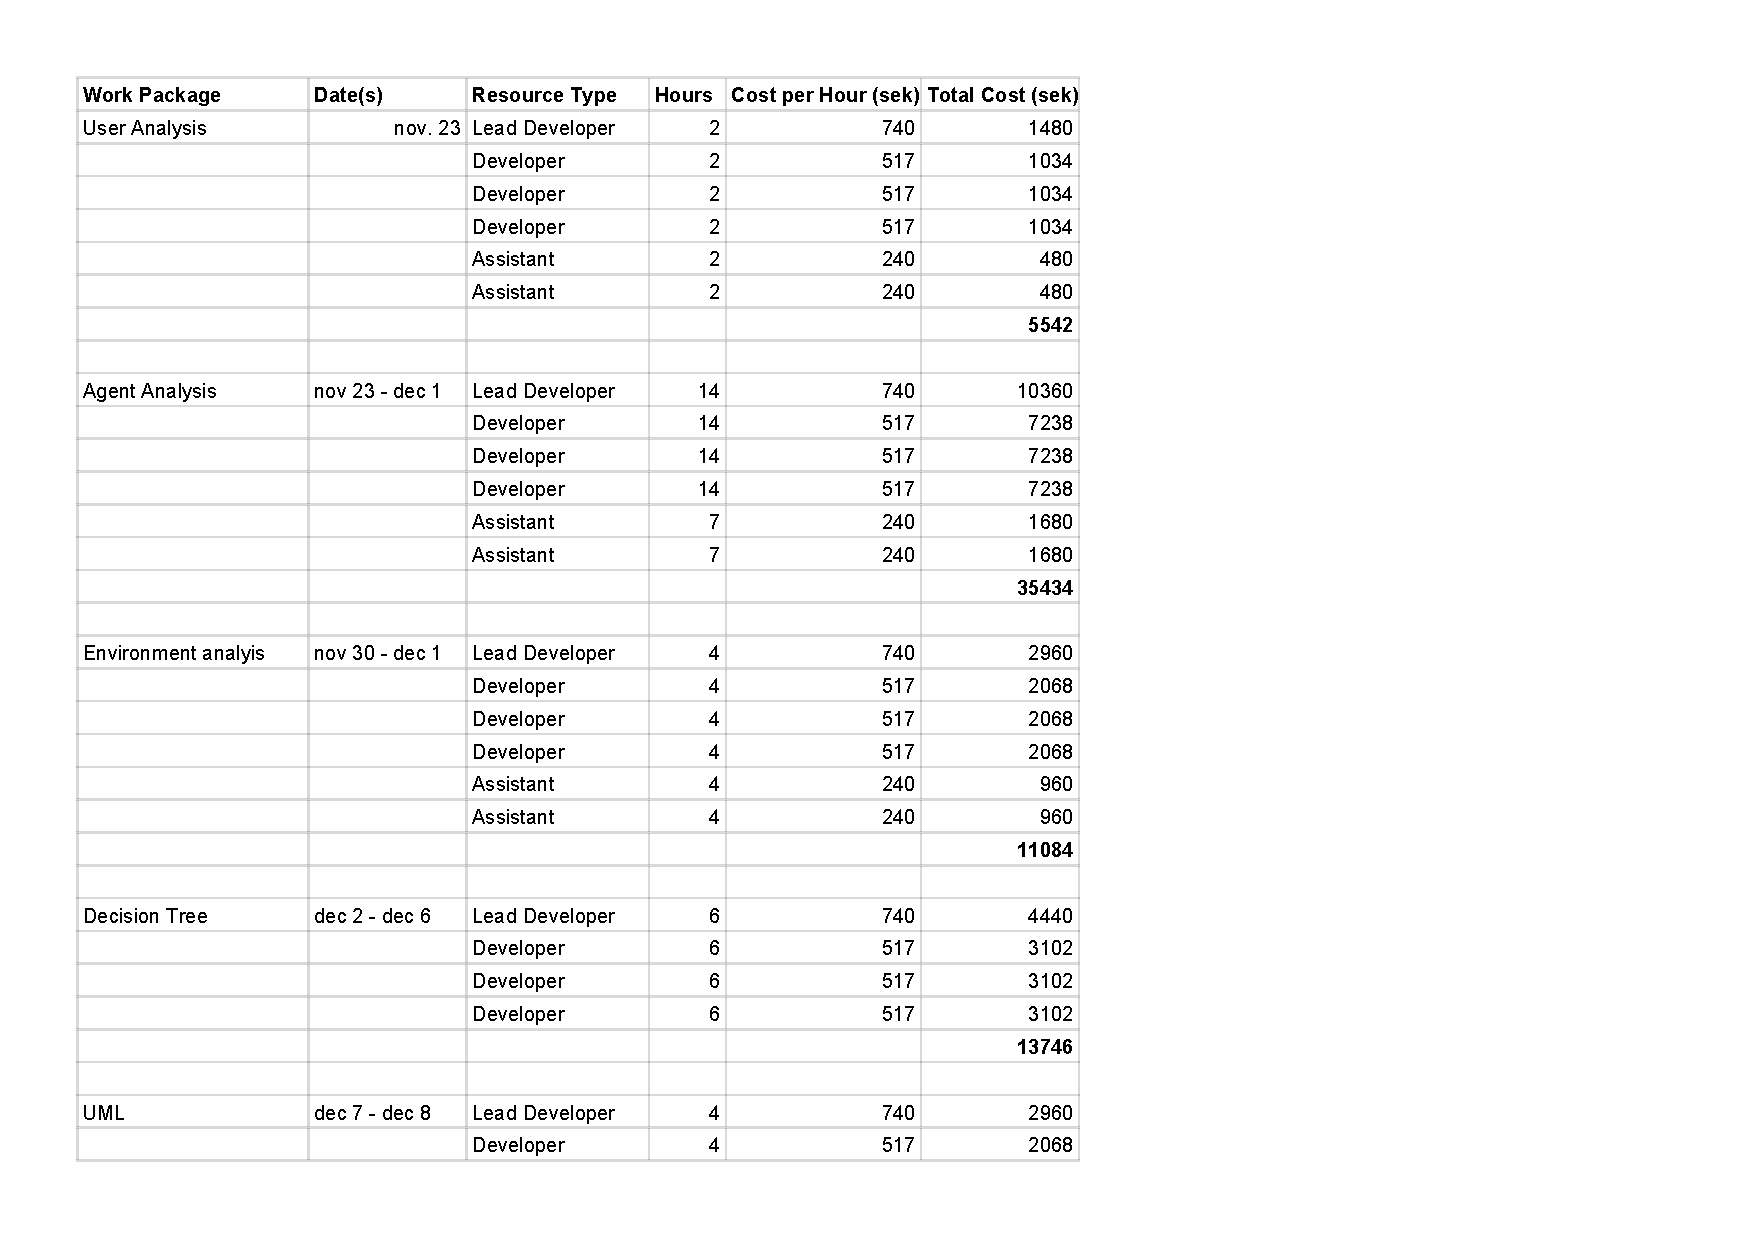
\includepdf[pages=-]{graphics/Resourceplan.pdf}

\end{document}
